\documentclass{standalone}
\usepackage{tikz}
\usepackage{ctex,siunitx}
\setCJKmainfont{Noto Serif CJK SC}
\usepackage{tkz-euclide}
\usepackage{amsmath}
\usetikzlibrary{patterns, calc,3d}
\usetikzlibrary {decorations.pathmorphing,decorations.pathreplacing,decorations.shapes}
\begin{document}
\small
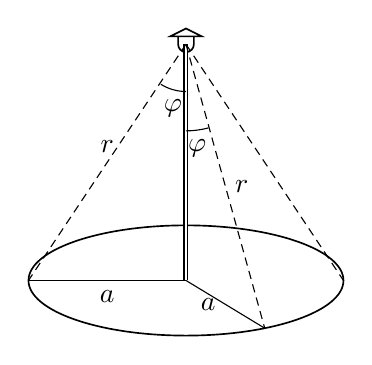
\begin{tikzpicture}[>=latex,scale=1.0]
  \draw[semithick](0,0)ellipse(2.0 and 0.7);
  \draw[semithick](-0.1,3.1)--(-0.1,3)arc(180:360:0.1)--++(0,0.1)(-0.2,3.1)--(0.2,3.1)--(0,3.2)--cycle;
  \draw[double distance=1pt](0,0)--(0,3);
  \draw[densely dashed](0,3)--(-2,0)node[midway,above]{$r$}(0,3)--(2,0);
  \draw[densely dashed](0,3)--({2*cos(60)},{-0.7*sin(60)})node[midway,right]{$r$};
  \draw(0,0)--(-2,0)node[midway,below]{$a$};
  \draw(0,0)--({2*cos(60)},{-0.7*sin(60)})node[midway,left]{$a$};
  \draw(0,2.4)arc(270:238:0.6)node[midway,below]{$\varphi$};
  \draw(0,1.9)arc(270:285:1.1)node[midway,below]{$\varphi$};
\end{tikzpicture}
\end{document}